
\chapter*{Introduction}
\label{sec:org7bf2d8d}

\section*{Motivation}
\label{sec:org83676f5}

\section*{Problem Statement}
\label{sec:org503778b}

\subsection*{Motivation}
\label{sec:orgffafb32}
\emph{Can some device run a given algorithm?}

\emph{How the mapping process affect the circuit "probability of success"?}

\begin{figure}[htbp]
\centering
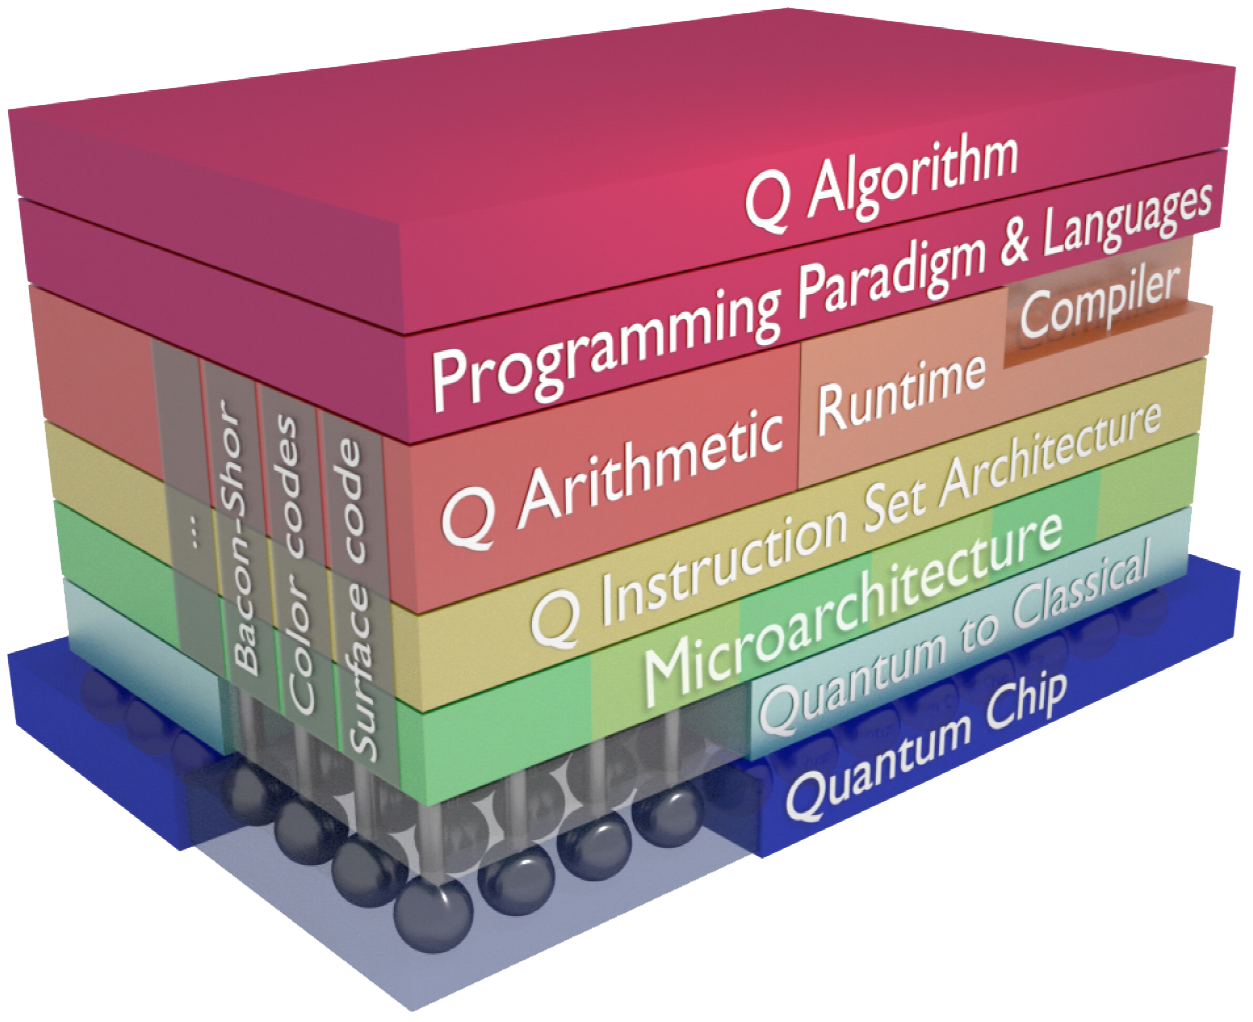
\includegraphics[width=0.7\textwidth]{figures/system_stack.png}
\caption{\label{fig:org22a0f4c}
Full stack implementation}
\end{figure}

\subsection*{Realization}
\label{sec:orgc7f25c2}
The work is centered in:

\begin{itemize}
\item SC-7 and SC-17 chips
\item Physical level, without error correction
\item Two error models:
\begin{itemize}
\item Pauli Noise (QX simulator)
\item Complex empirical error model (quantumsim)
\end{itemize}
\end{itemize}

\section*{Structure of the thesis}
\label{sec:org3ffc891}
